\section{Randomized Smoothing}

Given a classifier $f$ and $\epsilon \sim \No(0,\sigma^2 I)$, define a smoothed classifier $g$ as
$$g(x)=\argmax_c \P\left[f(x+\epsilon)=c\right].$$
\textbf{THM:} Suppose $\exists {p_A}, {p_B} \in [0,1]$, s.t. $\P\left[f(x+\epsilon)=c_A\right] \ge {p_A} \ge {p_B} \ge \max_{c\ne c_A} \P\left[f(x+\epsilon)=c\right].$ Then $g(x+\delta)=c_A$ for all $\|\delta\|_2 <R$, where the radius $R=\frac{\sigma}{2} (\Phi^{-1}({p_A})-\phi^{-1}({p_B}))$ and $\Phi^{-1}$ is the Gaussian quantile function.

If we have ${p_A}>\frac{1}{2}$, then ${p_B}\leq1-{p_A}<p_A$ and thus $R>\sigma \Phi^{-1}({p_A})$. To compute probability, we use sampling. To avoid selection bias, we first sample to get the top label and then use an independent sampling to estimate the probability:

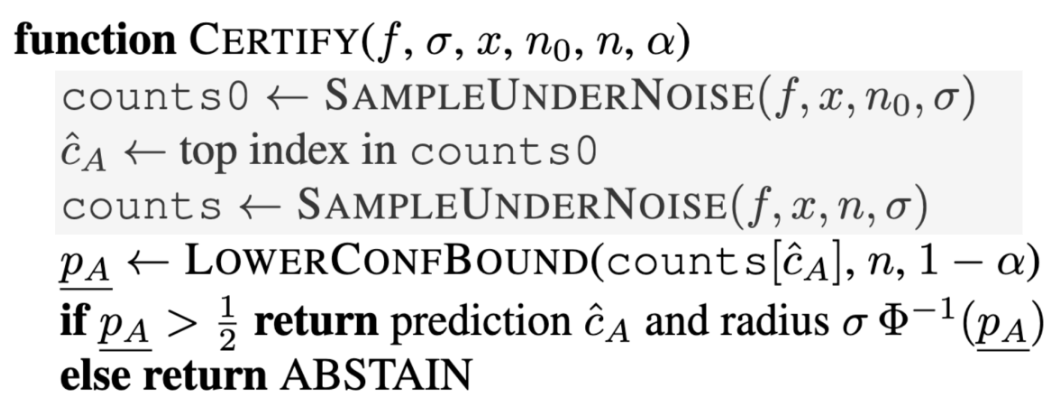
\includegraphics[width=\columnwidth]{img/rand_smooth.png}

By the above theorem, we have $g(x)=\hat{c}_A$ for all $\|\delta\|_2 <R$
with probability $1-\alpha$ if $\hat{c}_A, R$ is returned.

For inference, to compute $g(x)$, we use:

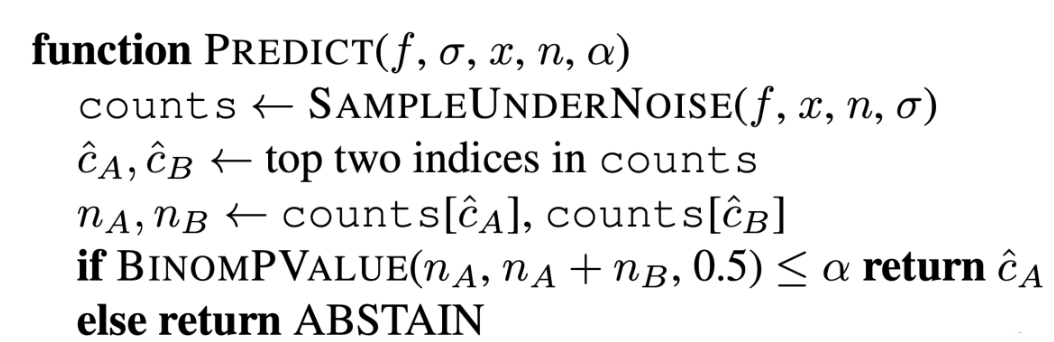
\includegraphics[width=\columnwidth]{img/rand-predict.png}

The probability of wrong prediction is $\P\left[\hat{c_A}\ne c_A, \text{no abstain}\right] = \P\left[\text{no abstain} \mid \hat{c_A}\ne c_A\right] \P\left[\hat{c_A}\ne c_A\right]\le \alpha$.

Pros: (1) it can scale to large networks and (2) is model-agnostic.

Cons: (1) it requires sampling at inference time and (2) many samples could be needed to increase the certified radius.